\documentclass{article}
\usepackage{graphicx}

\usepackage{amsmath}
\usepackage{amssymb}

\usepackage{cancel} %для сокращения слагаемых
%\usepackage{mathtools} %для красивого устремленя под пределами

\usepackage{graphicx} %Работа с картинками
\usepackage{wrapfig} % подписи к картинкам

\usepackage[T2A]{fontenc}
\usepackage[utf8]{inputenc}
\usepackage[russian]{babel}

\usepackage[%
  top=2.5cm,     % Верхнее поле
  bottom=2.5cm,  % Нижнее поле  
  left=3cm,      % Левое поле
  right=2cm      % Правое поле
]{geometry}

\title{
Проектная работа по Математическому анализу
\\ МатАн.Прод 11.1
\\ Вариант 3
}

\author{Веселов Фёдор, Группа 6}
\date{10.04.2026}

\begin{document}

\maketitle

\section{Индивидуальная часть}
\subsection{Составление интегральной суммы} 
\[f(x) = sinx, [0, \pi]\]
\[0 < x_1 < x_2 < ... < x_n < \pi\]
\[\Delta x_i = x_i - x_{i-1}\]
\[ \int_0^\pi f(x) \, dx \approx \sum_{i=1}^n f(\xi_i)\Delta x_i = 
\sum_{i=1}^n sin(\xi_i)\Delta x_i \]
\[ \text{Пусть, так как у нас разбиение равномерное, } \forall i,j: 
\Delta x_i = \Delta x_j \implies \Delta x_i = 
\frac{\pi - 0}{n} = \frac{\pi}{n}\]
\[\text{Пусть } \xi_i = x_i = i\cdot\frac{\pi}{n} = \frac{i\pi}{n}\]
\[\implies \sum_{i=1}^n sin(\frac{i\pi}{n})\cdot \frac{\pi}{n}
= \frac{\pi}{n}\sum_{i=1}^n sin(\frac{i\pi}{n})\]
\subsection{Нахождение интегральной суммы}
\[
\lim_{n \to \infty} \frac{\pi}{n}\sum_{i=1}^n sin(\frac{i\pi}{n}) =
\lim_{n \to \infty} \frac{\pi}{n}\sum_{i=1}^n \frac{sin(\frac{i\pi}{n})\cdot2sin(\frac{\pi}{n})}{2sin(\frac{\pi}{n})} \overset{(*)}{=}
\]
\[
(*): sin(\frac{i\pi}{n})\cdot2sin(\frac{\pi}{n}) = 
cos(\frac{i\pi}{n} - \frac{\pi}{2n}) - cos(\frac{i\pi}{n} + \frac{\pi}{2n})
= cos(\frac{\pi}{n}(i-\frac{1}{2})) - cos(\frac{\pi}{n}(i+\frac{1}{2}))
\]
\[
\overset{(*)}{=} \lim_{n \to \infty} \frac{\pi}{n}\cdot\frac{1}{2sin(\frac{\pi}{2n})}\cdot
\biggl(cos\Bigl(\frac{\pi}{n}\frac{1}{2}\Bigr) - \cancel{cos\Bigl(\frac{\pi}{n}\cdot\frac{3}{2}\Bigr)} + \cancel{cos\Bigl(\frac{\pi}{n}\cdot\frac{3}{2}\Bigr)}
- \cancel{...} + \cancel{cos\Bigl(\frac{\pi}{n}\cdot\frac{2n-1}{2}\Bigr)} - cos\Bigl(\frac{\pi}{n}\cdot\frac{2n+1}{2}\Bigr)\biggr) =
\]
\[
= \lim_{n \to \infty} \frac{\pi}{n}\Biggl( 
\frac{cos\Bigl(\frac{\pi}{2n}\Bigr) - cos\Bigl(\pi+\frac{\pi}{2n}\Bigr)}{2sin(\frac{\pi}{2n})} \Biggr) =
\lim_{n \to \infty} \frac{\pi}{n} \cdot 
\frac{\cancel{2}cos(\frac{\pi}{2n})}{\cancel{2}sin(\frac{\pi}{2n})}
= \lim_{n \to \infty} \underbrace{\frac{\frac{\pi}{2n}}{\sin(\frac{\pi}{2n})}}_{\to1} \cdot 
\underbrace{2\cos\left(\frac{\pi}{2n}\right)}_{\to 2} = 2
\]
\subsection{Доказательство того, что интеграл существует}
\[\text{Функция f(x) = sin(x) непрерывна на отрезке } [0,\pi] \text{, а следовательно по критерию}\]
\[\text{интегрируемости Римана она интегрируема} \implies 
\exists \int_0^\pi f(x) \, dx =  \int_0^\pi sin(x) \, dx \]

\subsection{Нахождение через определенный интеграл}
\[
\int_0^\pi f(x) \, dx = \int_0^\pi sin(x) \, dx = \Bigl[-cos(x)\Bigr]\Bigg|_0^\pi =
-\Bigl[cos(\pi) - cos(0)\Bigr] = -\Bigl[-1 - 1\Bigr] = 2 
\]
Значения интеграл вычисленные разными способами совпадают.

\subsection{Графики интегральных сумм}

\subsubsection{Метод левых прямоугольников}
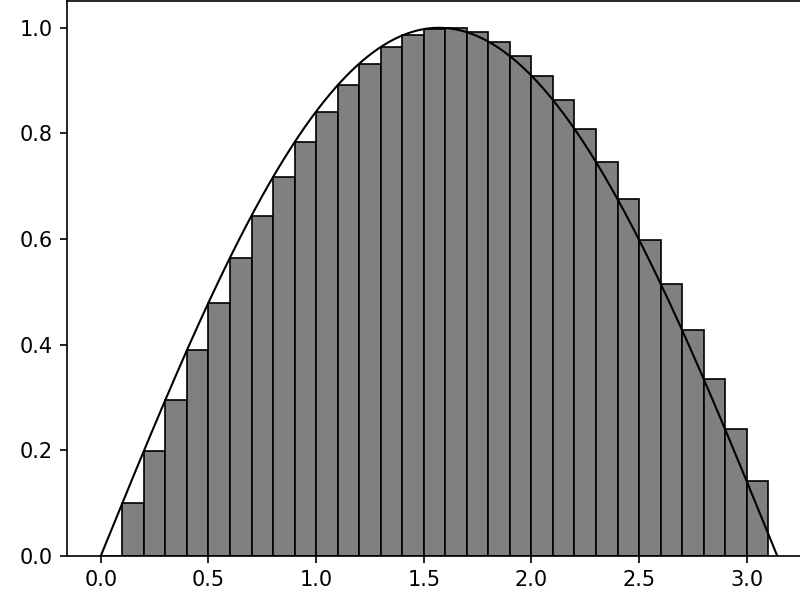
\includegraphics[width=0.5\textwidth]{Sin_left.png}
\\n = 31; Ранг разбиения: 0.1; S\textsubscript{гр} = 1.9953899
Формула погрешности для метода левых прямоугольников:
$$|R_n| \le \max_{x \in [a, b]} |f'(x)| \frac{(b - a)^2}{2n}$$
В нашем случае: 
$$|R_n| \le \max_{x \in [0, \pi]} |-sin(x)| \frac{\pi^2}{2n} = \frac{\pi^2}{2n} $$
$$ n = 31 \implies R_n \leq \frac{\pi^2}{62} < 0.15919$$ 
$$ |S_\text{ист} - S_\text{гр}| = 0,0046101 < 0,15 < R_n \implies \text{Рассчитано корректно}$$

\subsubsection{Метод правых прямоугольников}
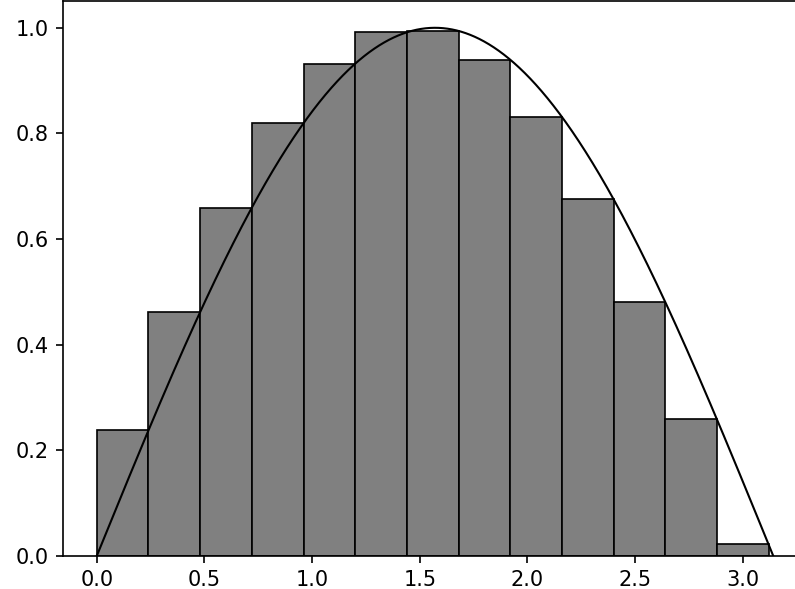
\includegraphics[width=0.5\textwidth]{Sin_right.png}
\\n = 13; Ранг разбиения: 0.24; S\textsubscript{гр} = 1.9927496961573818
Формула погрешности для метода правых прямоугольников(такая же):
$$|R_n| \le \max_{x \in [a, b]} |f'(x)| \frac{(b - a)^2}{2n}$$
В нашем случае: 
$$|R_n| \le \max_{x \in [0, \pi]} |cos(x)| \frac{\pi^2}{2n} = \frac{\pi^2}{2n} $$
$$ n = 13 \implies R_n \leq \frac{\pi^2}{26} < 0.37960017$$ 
$$ |S_\text{ист} - S_\text{гр}| = 0.007250304 < 0.008 < R_n \implies \text{Рассчитано корректно}$$

\subsubsection{Метод средних прямоугольников}
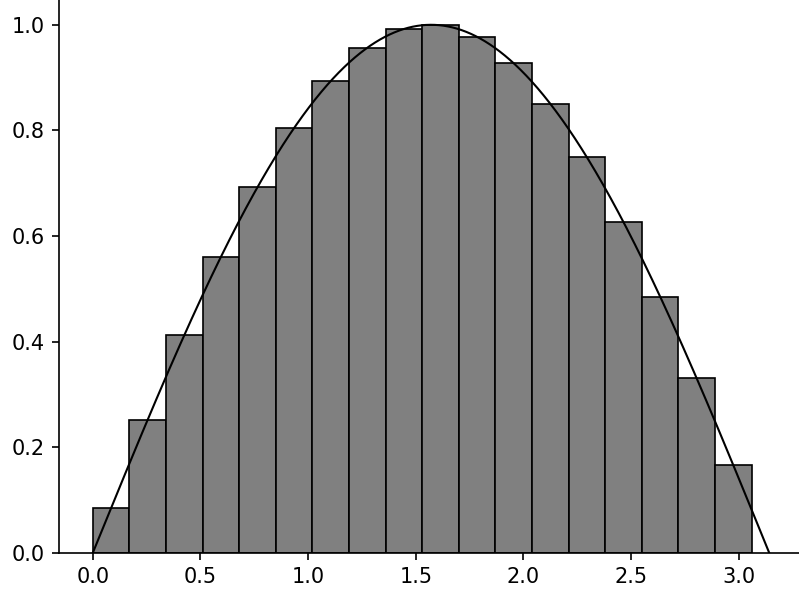
\includegraphics[width=0.5\textwidth]{Sin_middle.png}
\\n = 18; Ранг разбиения: 0.17; S\textsubscript{гр} = 1.9990795211790413
Формула погрешности для метода средних прямоугольников:
$$|R_n| \le \max_{x \in [a, b]} |f''(x)| \frac{(b - a)^3}{24n^2}$$
В нашем случае: 
$$|R_n| \le \max_{x \in [0, \pi]} |cos(x)| \frac{\pi^3}{24n^2} = \frac{\pi^3}{24n^2} $$
$$ n = 18 \implies R_n \leq \frac{\pi^3}{7776} < 0,003987432700656 $$ 
$$ |S_\text{ист} - S_\text{гр}| = 0.0009204788209587 < R_n \implies \text{Рассчитано корректно}$$

\subsubsection{Метод трапеций}
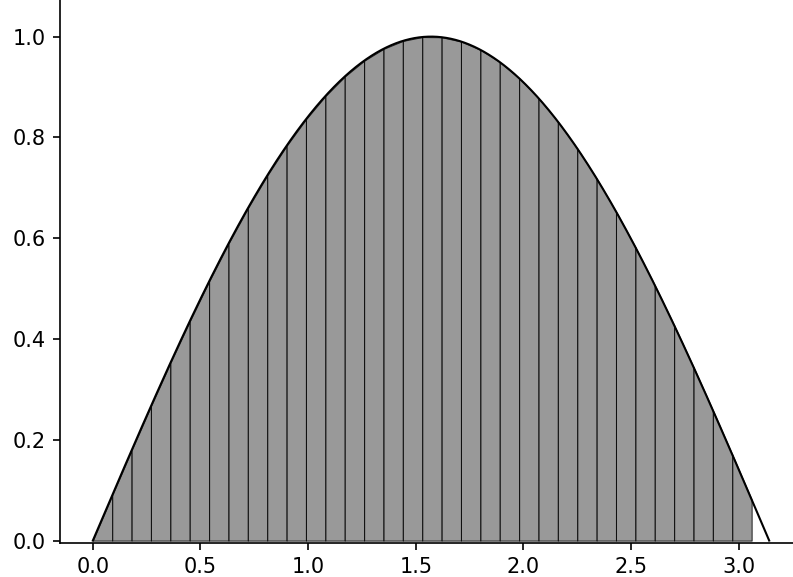
\includegraphics[width=0.5\textwidth]{Sin_trap.png}
\\n = 34; Ранг разбиения: 0.9; S\textsubscript{гр} = 1.9953252293472543
Формула погрешности для метода трапеций:
$$|R_n| \le \max_{x \in [a, b]} |f''(x)| \frac{(b - a)^3}{12n^2}$$
В нашем случае: 
$$|R_n| \le \max_{x \in [0, \pi]} |-cos(x)| \frac{(\pi - 0)^3}{12n^2} = \frac{\pi^3}{12n^2} $$
$$ n = 34 \implies R_n \leq \frac{\pi^3}{13872} < 0,0032351 $$ 
$$ |S_\text{ист} - S_\text{гр}| = 0.003174771 < R_n \implies \text{Рассчитано корректно}$$



\subsection{Нахождение погрешности оценки}
\[
\Delta = \Bigg| \int_0^\pi f(x) \, dx - S_n \Bigg| = \Bigg| 2 - \frac{\pi}{n}ctg\Bigl(\frac{\pi}{2n}\Bigr) \Bigg|
\]
\[
\text{Теориетиеская погрешность: } |R_n| \leq \max_{x \in [0,\pi]}|f'(x)|\frac{(\pi-0)^2}{2n}
= \max_{x \in [0,\pi]}\Bigl[\frac{\pi^2}{2n}cos(x)\Bigr] = \frac{\pi^2}{2n}  
\]
Использем разложение котангенса в ряд Лорана в окрестности нуля:
\[ \cot(t) = \frac{1}{t} - \frac{t}{3} - \frac{t^3}{45} + O(t^5) \]
Подставим $t = \frac{h}{2}(h=\pi x=\frac{\pi}{n})$:
\[ \Delta(h) = \left| 2 - h \left( \frac{1}{h/2} - \frac{h/2}{3} + O(h^3) \right) \right| \]
\[ \Delta(h) = \left| 2 - \left( 2 - \frac{h^2}{6} + O(h^4) \right) \right| \]
\[ \Delta(h) = \frac{h^2}{6} + O(h^4) \implies\]
\[R_n \sim O(\frac{1}{n})\]
\[\Delta \sim O(\frac{1}{n^2})\]
\\
\\
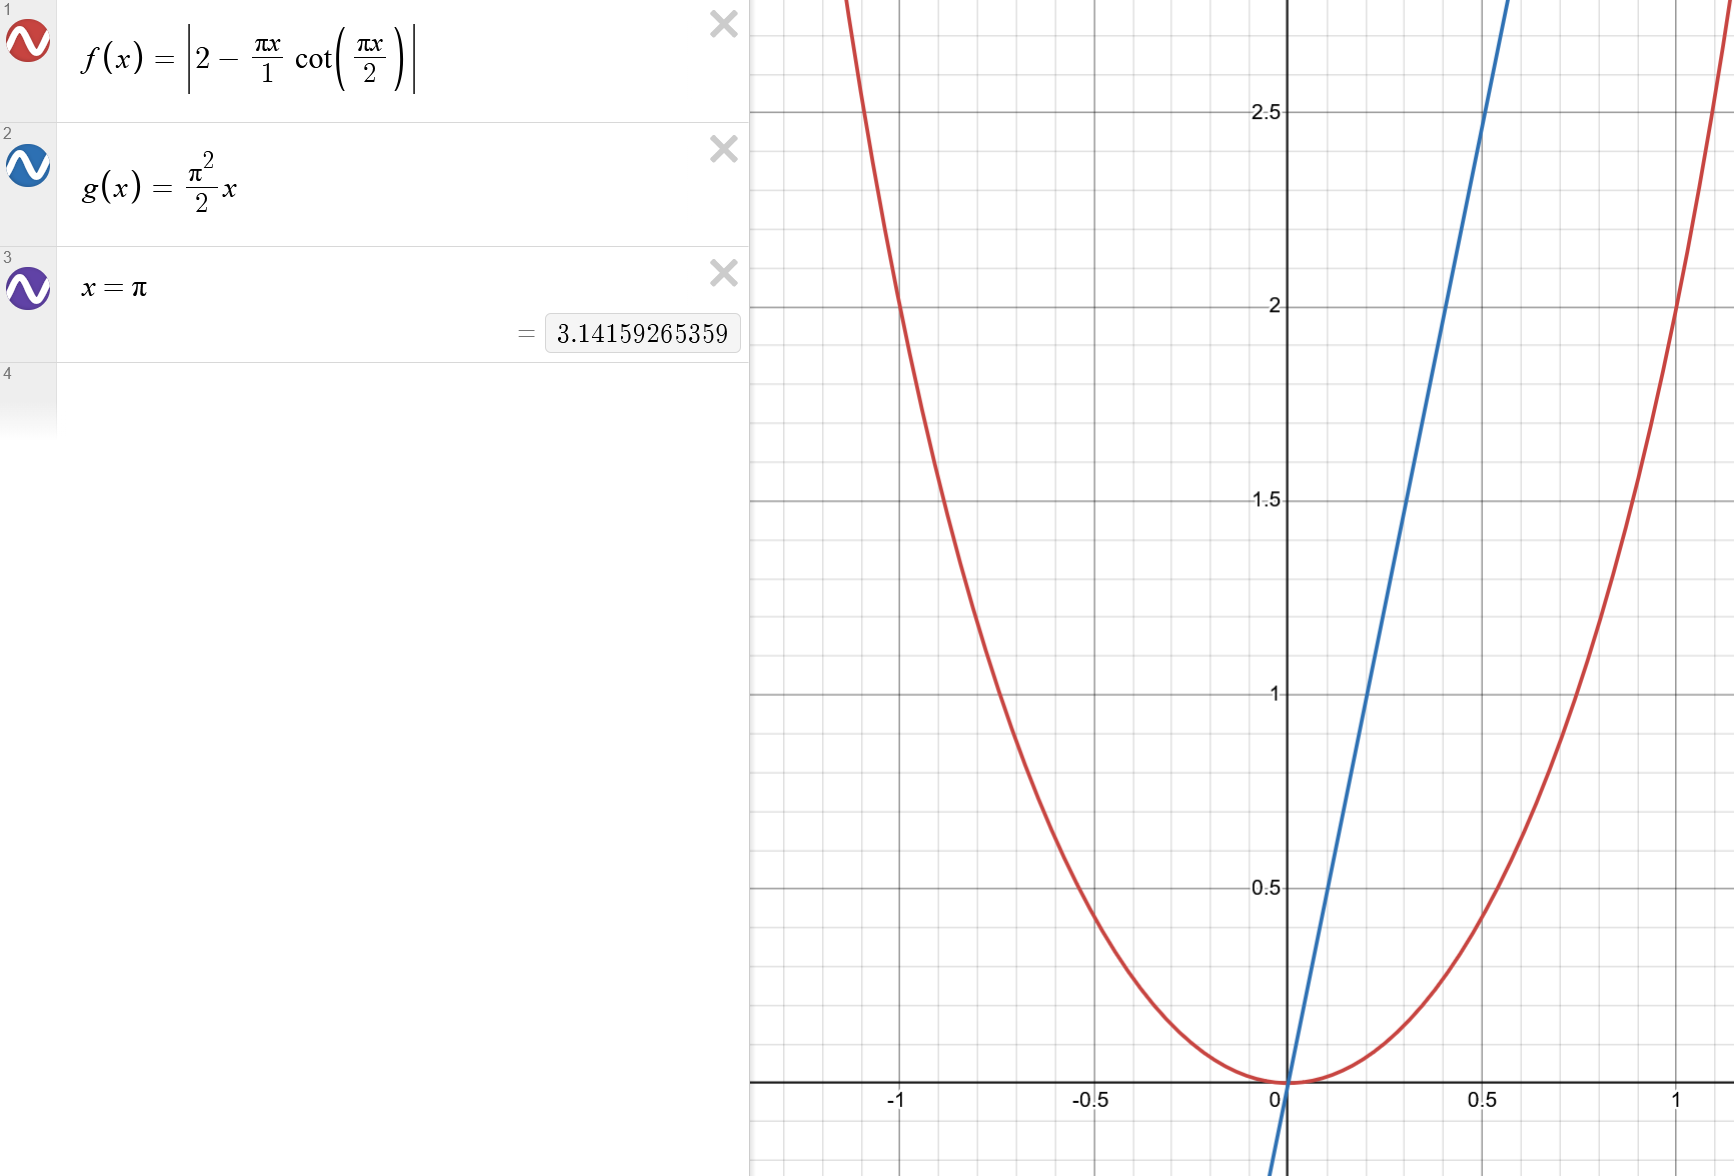
\includegraphics[width=0.8\textwidth]{Погрешности.png}

\[\text{Графики погрешностей при } n\to\infty \text{ }(x\to0)\] 


\include{part2}
\end{document}
